%!TEX root = fastZKP.tex
\section{Linear Prover Time GKR Protocol}
In this section, we will present an implementation of GKR protocol\cite{GKR}, which is a improved version of CMT protocol\cite{CMT}. In this section we will improve the original CMT protocol and then propose slightly modified verion of improved CMT to make it zero knowledge.

\subsection{Roadmap}
Through out the whole CMT protocol, the prover has to answer two type of queries, one is the query related to sumcheck, another one is the query to combine the points. We will deal with these queries seperately. The equation in sumcheck queries are well structured. For each sumcheck we are going to check the claim $a_i=\tilde{V_i}(r_i)$ where $\tilde{V_i}(r_i)=\sum_{g\in\{0,1\}^{s_i} u, v\in \{0,1\}^{s_{i+1}}}f_{i,r_i}(g,u,v)$. Since the sumcheck deal with the parameters one by one, we can divide the sumcheck into three stages as follows: $\tilde{V_i}(r_i)=\sum_{g\in\{0,1\}^{s_i}}\sum_{u \in \{0,1\}^{s_{i+1}}} \sum_{v\in \{0,1\}^{s_{i+1}}}f_{i,r_i}(g,u,v)$, where $f_{i,r_i}(g,u,v)\overset{def}{=}\tilde{\beta_{i}}(r_i, g)[\tilde{mult}(g, u, v)(\tilde{V}_{i+1}(u)\tilde{V}_{i+1}(v))+\tilde{add}(g,u,v)(\tilde{V}_{i+1}(u)+\tilde{V}_{i+1}(v))]$, the first stage is the summation of $g$, the second and the third stage is the summation of $u$ and $v$. Also notice that $\tilde{mult}$ and $\tilde{add}$ are independent in the equation, independent means that we can calculate them seperately and the final answer is the sum of these two. So we can treat them seperately using two similar algorithm.

For simplicity, in this subsection we only discuss the idea of calcuate $\tilde{mult}$ part. our simplified equiation becomes 
$$a_{i_{mult}}=\sum_{g\in\{0,1\}^{s_i}}\sum_{u \in \{0,1\}^{s_{i+1}}} \sum_{v\in \{0,1\}^{s_{i+1}}}f_{i, r_i}(g, u, v)$$ where $$f_{i, r_i}(g, u, v)=\tilde{\beta_{i}}(r_i, g)\tilde{mult}(g, u, v)(\tilde{V}_{i+1}(u)\tilde{V}_{i+1}(v))$$


During the sumcheck, the verifier will asks a univariate function. In the first stage $i$-th round, the univariate function would be: $f_i(x_i)=\sum_{g_{i+1} \in \{0, 1\}, ..., g_{s_{i}} \in \{0, 1\}} \sum_{u} \sum_{v} \tilde{\beta_{i}}(r_i, g')\tilde{mult}(g', u, v)(\tilde{V}_{i+1}(u)\tilde{V}_{i+1}(v))$, where $g' = a_1, a_2, ..., a_{i-1}, x_{i}, g_{i+1}, ..., g_{s_i}$, $a_i$ is the random number in earlier rounds from the verifier. Clearly $x_i$ appears in two subfunctions: $\tilde{\beta}$, $\tilde{mult}$. The univariate function is the product of two 1-degree polynomial. The idea is to calculate the coefficient of these 1-degree polynomials. This observation also apply for the second and third stage. A 1-degree polynomial can be determined by two points. In the binary tree, we node represent a single 1-degree polynomial, and we ensure that the child's polynomial will equals to father's polynomial when the inputs are either \{0, 1\}. If it's left child, they agree on input $0$, and if it's right child, they agree on $1$.

Combining two points is a relatively easy part, we will directly discuss the detailed algorithm in next subsection.

\subsection{Detailed Protocol}
\subsubsection{Binary tree structrue}
In the whole algorithm, we will construct a $s_i$-depth binary tree to process $g$, a $s_{i+1}$-depth binary tree for $u$, a $s_{i+1}$-depth binary tree for $v$. Each binary tree node represents two $1$-degree polynomials. They share the same structure, but the initialization is different for each tree. 

In this subsection , we will use $g$'s two binary trees as example, one tree describes the $1$-degree polynomial generated by $\tilde{\beta}$ fucntion, another one tree describes the $1$-degree polynomial generated by $\tilde{mult}$. 

In figure \ref{fig::bin_structure}, the root represent the polynomial used in the last step of sumcheck. The left child of the root represent the polynomials $\tilde{\beta}(z, (r_1, r_2, ..., r_{s-2}, x, 0))$, $\sum_{u, v}\tilde{mult}(z, (r_1, r_2, ..., r_{s-2}, x, 0), u, v)$ and it's similar for the right child. Let $L_{k, j, \tilde{\beta}}(x), L_{k, j, \tilde{mult}}$ be polynomials represented by $j$-th node with depth $s_i - k$ where $k=0$ represents leaves. $child_{k, j, 0}, child_{k, j, 1}$ be it's left and right child. 

For $k \ge 1$, we have $L_{k, j, \tilde{\beta}}(0)=L_{k-1, child_{k, j, 0}}(r_{k-1})$ and $L_{k, j, \tilde{\beta}}(1)=L_{k-1, child_{k, j, 1}}(r_{k-1})$, having these two points, we can get the $1$-degree polynomial in constant time. We can conclude that if we can initialize the leaf nodes, we can calculate the whole tree in linear time.

For each $k$-th sumcheck query, the answer would be $\sum_{j}(L_{k, j, \tilde{\beta}}(x)L_{k, j, \tilde{mult}}(x))$, we can calculate it by scanning through the $s_i-k$-th layer of the binary tree. The whole sumcheck for the first stage costs linear time for scanning the binary tree if we can initialize the values in the leaf in linear time.

\begin{figure}
\label{fig::bin_structure}
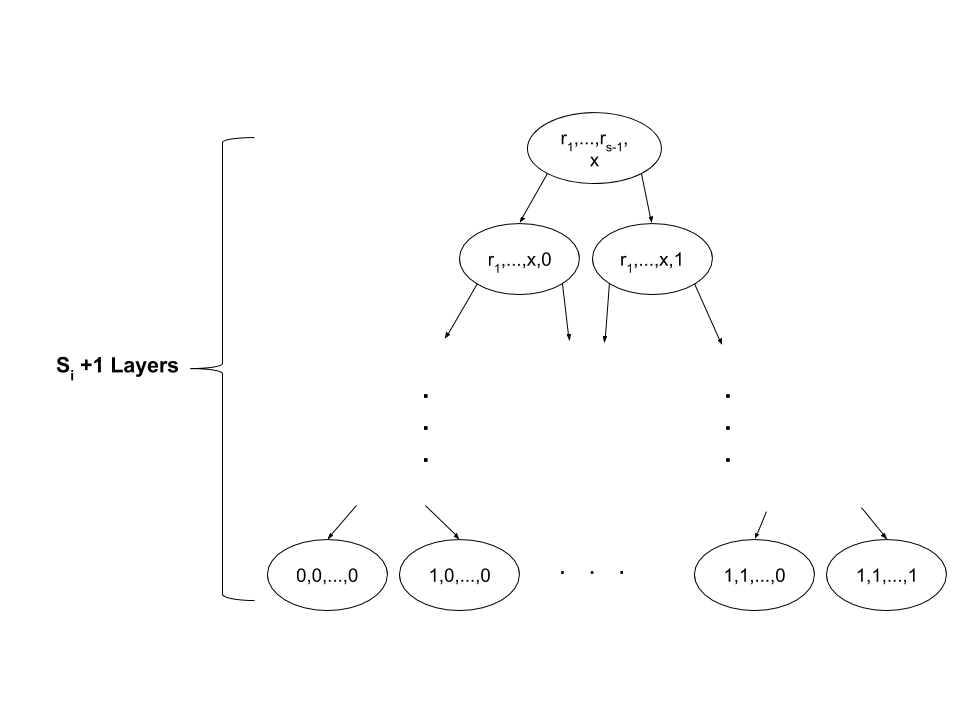
\includegraphics[width=15cm]{structurebintree.png}
\caption{The structure of the binary tree, each tree node stores a $1$-degree polynomial, and the leaf degenerate to constant.}
\end{figure}

\subsubsection{First Stage Preprocessing}

\subsection{Running Time Analysis}